\section{Planing}
In the first phase of the project the group spent a couple of days where we went through the stages of the project that we knew, or expected, would be needed. We estimated how long the different staged would take, which can be seen in the roadmap in figure \ref{fig:roadmap}.
 
\begin{figure}[h]
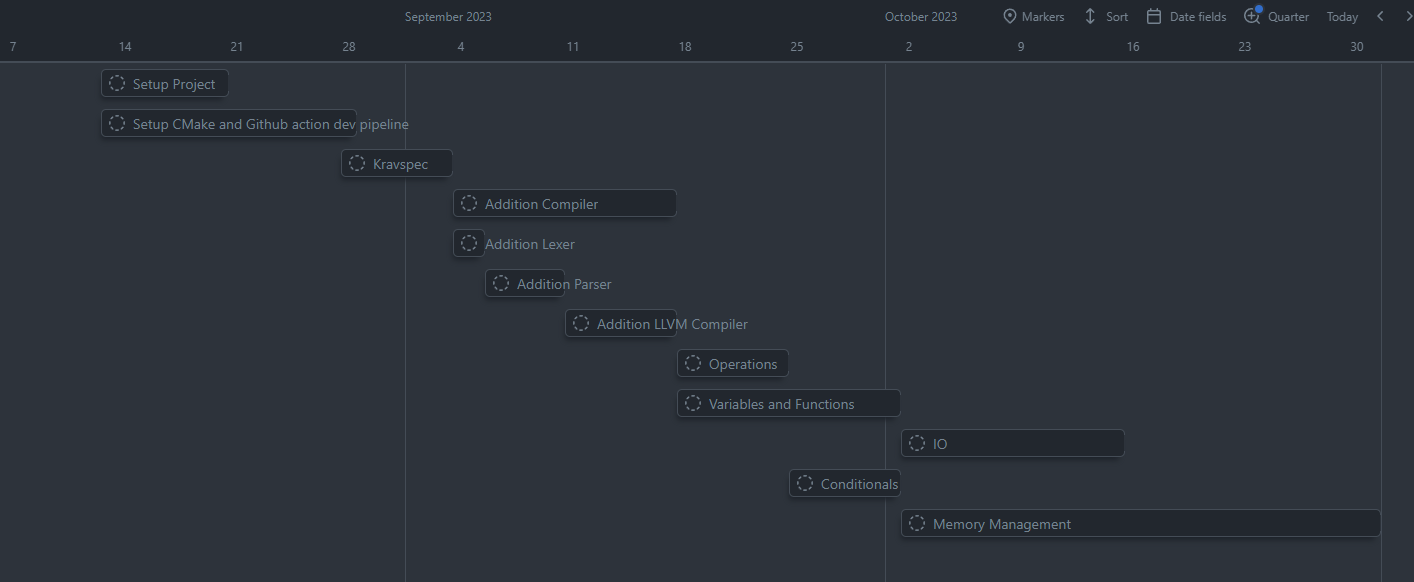
\includegraphics[width=\textwidth]{02-Body/Images/Roadmap.png}
\label{fig:roadmap}
\caption{Roadmap plan for the entire development}
\end{figure}

The roadmap starts with small, somewhat easily comprehended tasks, and tuns into more general tasks, spanning longer time. This is deliberate, as we expected to gain new knowledge in the process, and rather than having to continually rework the roadmap, we found it more convenient to define overall phases and deadlines, and leave the detailed planing until we had the experience of the preceding tasks.\\
It may be noticed that the roadmap contains two tasks for the majority of the development phase. This is because we from the beginning decided that we would be best served by working on tasks in parallel, preferably so diverse that they wouldn't cause conflicts in git. No thought was at this time given to who would undertake which task, nor was it expected that the tasks and time frames would remain unchanged (as indeed they were not).

